\begin{frame} %%% DEM
\frametitle{Discrete Euler-Maruyama (DEM)}
Method:
\begin{equation*}
	\left \{
	\begin{aligned}
		X_h^d(t_{i+1}) &= f(X(t_i))h + g(X(t_i))(W(t_{i+1}) - W(t_{i})),  \\
		X_h^d(0) &= X_0.
	\end{aligned} \right .
\end{equation*}
Parameters of interest computed naively
\begin{equation*}
\begin{aligned}
	\tau_h^d &= \min\{\tau_{h,e}^d,T\}, \text{ where } \tau_{h,e}^d = \min \{t_i \colon X_h^d(t_i) \notin D\}, \\
	\phi_h^d &= \mathbbm{1}_{\{T < \tau_{h,e}^d\}}F(X_h^d(T)).
\end{aligned}
\end{equation*}
Missed exits $\Rightarrow$ 1/2 loss in weak order:
\begin{align*}
	|\mathbb{E}(\tau_h^d) - \mathbb{E}(\tau)| &= O(\sqrt{h}), \\
	|\mathbb{E}(\phi_h^d) - \mathbb{E}(\phi)| &= O(\sqrt{h}).
\end{align*}	
\end{frame}

\begin{frame} %%% CEM 
\frametitle{Continuous Euler-Maruyama (CEM)}
\underline{Goal}. Restore the weak order of convergence 1 of Euler-Maruyama $\Rightarrow$ Brownian bridge approach.

Method:
\begin{equation*}
	\left \{
	\begin{aligned}
		X_h^c(t) &= f(X(t_i))(t-t_i) + g(X(t_i))(W(t) - W(t_{i})),  && t_i < t \leq t_{i+1},\\
		X_h^c(0) &= X_0.
	\end{aligned} \right .
\end{equation*} 
Estimate at each time step the probability of exit. If $D$ is an half-space
\begin{equation*}
\begin{aligned}
	&\Pr (\exists t \in [ t_i,t_{i+1} ] \quad X_h^d(t) \notin D | X_h^d(t_i) = x_i, X_h^d(t_{i+1}) = x_{i+1}) \\
	&\quad = p(x_i,x_{i+1},h) \\
	&\quad = \exp\Big(-2\frac{[n\cdot(x_i - z_i)][n\cdot(x_{i+1} - z_i)]}{hn\cdot (gg^T(x_i)n)}\Big).
\end{aligned}
\end{equation*}
\end{frame}

\begin{frame}
\frametitle{Continuous Euler-Maruyama (CEM)}
Parameters of interest. Given $u$ a realization of $U$ uniform r.v. in $(0,1)$
\begin{equation*}
\begin{aligned}
	\tau_h^c &= \min \{T,\tau_{h,e}^c\}, \\
	\text{ where } \tau_{h,e}^c &= \min\{\tau_{h,e1}^c, \tau_{h,e2}^c\}, \\
	\tau_{h,e1}^c &= \min\{t_i = hi \colon X_h(t_i) \notin D\}, \\
	\tau_{h,e2}^c &= \min\{t_i = hi \colon u < p(x_{i-1},x_i,h) \}, \\
	\phi_h^c &= \mathbbm{1}_{\{T < \tau_{h,e}^c\}}F(X_h^c(T)).
\end{aligned}
\end{equation*}
Weak order 1 is restored:
\begin{align*}
	|\mathbb{E}(\tau_h^c) - \mathbb{E}(\tau)| &= O(h), \\
	|\mathbb{E}(\phi_h^c) - \mathbb{E}(\phi)| &= O(h).
\end{align*}
\end{frame}

\begin{frame} %%% Adaptivity
\frametitle{An adaptive procedure}
\underline{Goal}. Restore the weak order of convergence 1 of Euler-Maruyama $\Rightarrow$ Adaptivity in space. \\
\underline{Setting}. Consider $\sigma \in \R$, $I$ the identity in $\R^{d \times d}$ and
\begin{equation*}
\left \{
\begin{aligned}
	dX(t) &= f(X(t)) dt + \sigma I dW(t), && 0 < t \leq T, \\
	X(0)  &= X_0, && X_0 \in D.
\end{aligned} \right .
\end{equation*}
\underline{Idea}. Given $l \in \N, h_0 > 0$, adapt step size $h$ in DEM as follows
\begin{equation*}
	h = \max\Big\{ h_{bound}, \min\Big\{ h_{int}, \Big(\frac{d}{(l + 3)\sigma}\Big)^2\Big\}\Big\}.
\end{equation*}
where
\begin{equation*}
\begin{aligned}
	h_{bound} &= 2^{-2l}h_0, \\
	h_{int} &= 2^{-l}h_0.
\end{aligned}
\end{equation*}
\end{frame}

\begin{frame}
\frametitle{An adaptive procedure}
\begin{minipage}[0]{0.49\linewidth}
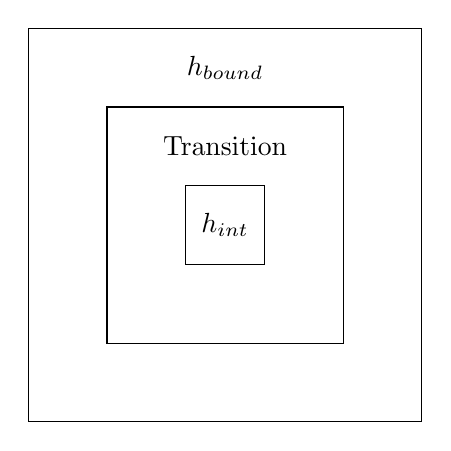
\begin{tikzpicture}
	\draw (0,0) rectangle (5,5);
	\draw (1,1) rectangle (4,4);
	\draw (2,2) rectangle (3,3);
	\node[align=center] at (2.5, 2.5) {$h_{int}$};
	\node[align=center] at (2.5, 3.5) {Transition};
	\node[align=center] at (2.5, 4.5) {$h_{bound}$};
\end{tikzpicture}
\end{minipage}
\begin{minipage}[0.5]{0.49\linewidth}
Quel porco di mazzinga la vede.
\end{minipage}

\end{frame}



